Molecular modeling seeks to gain new insights into the real world behavior of molecules by mimicking these molecules using computer simulations.
According to the theory of ``minimal frustration'', evolution selectively favors proteins sequences which fold to a stable native state, contained within a broad potential energy well, with a minimum number of possible non-native mis-folded conformations \cite{bryngelson1987spin}.
Thus, the prediction of native or native-like conformations focuses on finding those conformations which have a low potential energy.
As measuring the true potential energy of a system is very difficult or impossible, computational models seek to reproduce the qualitative behavior of the protein potential energy surface.

Quantum mechanics calculations are often viewed as the gold standard with respect to intramolecular energy calculations.
However, despite its accuracy, applying quantum mechanics to large systems such as proteins is currently impossible due to the amount of time necessary to perform quantum mechanics calculations on such a large number of atoms, as indicated in figure \ref{figure:conservation_of_annoyance}.
\begin{figure}[h]
\begin{center}
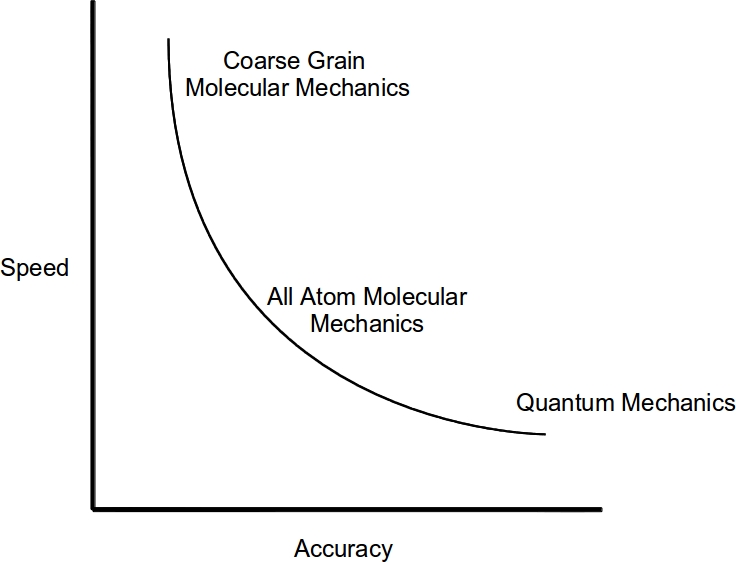
\includegraphics[width=0.7\textwidth]{figures/conservation_of_annoyance.png}
\caption{To an extent it is always possible to either increase accuracy or decrease running time, i.e. the cost of an experiment.
New scientific methods should allow one to increase accuracy while not spending additional time performing computations.}
\label{figure:conservation_of_annoyance}
\end{center}
\end{figure}
Instead, quantum mechanics calculations have been used to parameterize a majority of the most popular molecular mechanics force fields currently in use, including:
\begin{enumerate}
\item AMBER \cite{weiner1984new},
\item OPLS-AA \cite{kaminski1994free},
\item and CHARMM \cite{mackerell2002charmm}.
\end{enumerate}
These force fields all include covalent and non-covalent parameters which have been fit to quantum mechanics experiments.

The earliest molecular mechanics force fields were largely coarse grained, modeling groups of atoms as a unit, hydrogens grouped with their bound heavy atom \cite{jorgensen1988opls}, or each residue as a unit \cite{lee1999energy}, both to reduce the number of parameters in the model and to increase the speed of computations.
Although {\it ab initio} folding experiments are theoretically interesting, they are generally not practical because of the difficulty in simulating such a large system for the time-frame necessary to observe behaviors like folding, and also because structural models for many proteins are available either directly as X-ray structures, or indirectly through homology.

Because of the evolutionary cost of misfolding, proteins have been selected to minimize misfolding, making the general shape of the potential energy surface roughly funnel-like, with the native structure at the minimum \cite{leopold1992protein}.
Despite this shape, the energy landscape of proteins is a very jagged surface, with a large number of local minima \cite{tsai1999folding}.
These shapes, as well as the effect of solvation on smoothing the energy surface are illustrated in figure \ref{fig:funnel}.

\begin{figure}[h]
\centering
\begin{subfigure}[b]{0.3\textwidth}
    \centering
    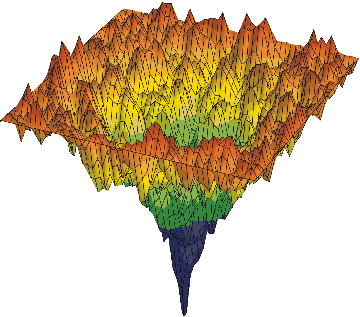
\includegraphics[width=\textwidth]{figures/drysurf.png}
    \label{fig:dry}
    \caption{}
\end{subfigure}%
\hspace{0.1\textwidth}
\begin{subfigure}[b]{0.3\textwidth}
    \centering
    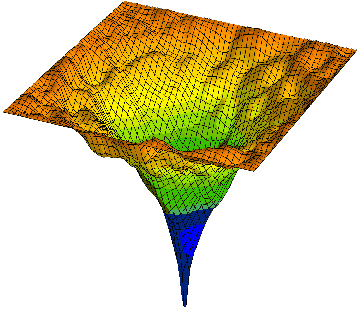
\includegraphics[width=\textwidth]{figures/wetsurf.png}
    \label{fig:wet}
    \caption{}
\end{subfigure}
\caption{
The protein energy surface is roughly funnel shaped.
Figure from \protect\cite{waterwebsite} used with authors permission.
}
\label{fig:funnel}
\end{figure}


Even the smallest enzyme contains 62 amino acids, and has thousands of degrees of freedom \cite{chen19924}, and larger enzymes are regularly more than 1000 amino acids in length.
The number of degrees of freedom of these systems make any attempt to analytically solve for a global minimum energy conformation impossible, and instead require other methods of generating plausible conformations.
In order to compensate for this, a number of different sampling methods have been developed.
